\documentclass[11pt,a4paper]{article}

% =========================
% Encoding & Fonts (pdflatex-safe)
% =========================
\usepackage[utf8]{inputenc}
\usepackage[T1]{fontenc}
\usepackage{lmodern}

% =========================
% Layout
% =========================
\usepackage[a4paper,margin=1.5cm]{geometry}
\setlength{\parindent}{0pt}
\setlength{\parskip}{6pt}

% =========================
% Packages
% =========================
\usepackage{amsmath,amssymb}
\usepackage{enumitem}
\usepackage{hyperref}
\usepackage{xcolor}
\usepackage{listings}
\usepackage{titlesec}
\usepackage{fancyhdr}
\usepackage{tabularx}
\usepackage{array}
\usepackage{graphicx}
\usepackage{tikz}
\usetikzlibrary{calc}
\usetikzlibrary{arrows.meta}

% =========================
% Header / Footer
% =========================
\pagestyle{fancy}
\fancyhf{}
\lhead{\textbf{Lebanese University -- Faculty of Engineering}}
\rhead{\textbf{Semester VIII}}
\cfoot{\thepage}

% =========================
% Section formatting
% =========================
\titleformat{\section}{\Large\bfseries}{\thesection.}{0.5em}{}
\titleformat{\subsection}{\large\bfseries}{\thesubsection.}{0.5em}{}
\titleformat{\subsubsection}{\normalsize\bfseries}{\thesubsubsection.}{0.5em}{}

% =========================
% Code style
% =========================
\lstset{
	basicstyle=\ttfamily\small,
	frame=single,
	breaklines=true,
	columns=fullflexible,
	keywordstyle=\color{blue},
	commentstyle=\color{gray},
	stringstyle=\color{red},
	showstringspaces=false
}

% =========================
% Helpers
% =========================
\newcommand{\courseTitle}{Concurrency \& Distributed Systems}
\newcommand{\courseSubtitle}{Diagnosing Broken Systems: From Threads to Clusters}
\newcommand{\primaryLang}{Java}
\newcommand{\counterWeek}{Python (with brief Go/Erlang contrast)}
\newcommand{\level}{Senior Undergraduate / Graduate}
\newcommand{\format}{Theory + Failure-Driven Labs + Evolving Project + Presentations}
\newcommand{\instructor}{Dr. Mohamad Aoude}

\begin{document}
% ============================================================
% Week 1 Lecture Plan — Why Concurrency Exists (Pain First)
% IMPROVED VERSION (Two-Session Format)
% ============================================================

\subsection*{Week 1 Lecture Plan --- Why Concurrency Exists (Pain First)}
\textbf{Improved Version}

\vspace{2mm}
\hrule
\vspace{3mm}

% ------------------------------------------------------------
\subsubsection*{Pre-Class Preparation (Instructor)}

\textbf{Essential materials to prepare:}
\begin{itemize}[leftmargin=*]
	\item[$\square$] Working demo server code (single-threaded + multi-threaded versions)
	\item[$\square$] Load testing client (pre-configured for 10, 50, 100 concurrent clients)
	\item[$\square$] Monitoring dashboard or terminal setup showing CPU/latency in real-time
	\item[$\square$] Pre-recorded backup demos (in case live demo fails)
	\item[$\square$] Lab 1.1 starter code repository ready for distribution
\end{itemize}

\textbf{Room setup:}
\begin{itemize}[leftmargin=*]
	\item Projector showing: terminal output + system monitor side-by-side
	\item Backup laptop for demos (Murphy's Law)
\end{itemize}

% ------------------------------------------------------------
\subsubsection*{Learning Targets (Concrete \& Measurable)}

By the end of Week 1, students must be able to:

\begin{enumerate}[leftmargin=*]
	\item \textbf{Explain} the difference between latency and throughput with a concrete example
	\item \textbf{Predict} when adding threads will help vs hurt (given a workload profile)
	\item \textbf{Measure} both metrics using basic tooling and report them accurately
	\item \textbf{Diagnose} why a server feels slow despite low CPU usage
	\item \textbf{Articulate} the ``waiting problem'' that concurrency solves
\end{enumerate}

\textbf{Assessment checkpoint:} Exit ticket (5 questions, 2 minutes)

% ------------------------------------------------------------
\subsubsection*{Enhanced Structure: Two-Session Format (Recommended)}

% ============================================================
\paragraph{Session 1 (2h) --- ``The Pain \& The Problem''}

\subparagraph{0) Hook + Course Context (5 min)}
\textbf{Opening question (silent thinking):}\\
\textit{``Why does your phone browser load 10 tabs simultaneously, but your backend can only handle requests one at a time?''}

\textbf{Course promise callback:}\\
\textit{``By Week 14, you'll diagnose production failures. Today, we learn why systems fail under load.''}

\textbf{Session roadmap (on board):}
\begin{verbatim}
	Today's journey:
	1. Watch a server die
	2. Understand why it died
	3. Fix it (partially)
	4. Watch it die again (differently)
\end{verbatim}

\subparagraph{Conceptual Model: Why Waiting Exists}

Every program alternates between:

\begin{itemize}
	\item CPU computation
	\item Waiting (I/O, network, disk, locks)
\end{itemize}

If a program waits 90\% of the time, then:

\begin{center}
	The CPU is idle 90\% of the time.
\end{center}

Concurrency exists to exploit idle waiting time.
\begin{center}
	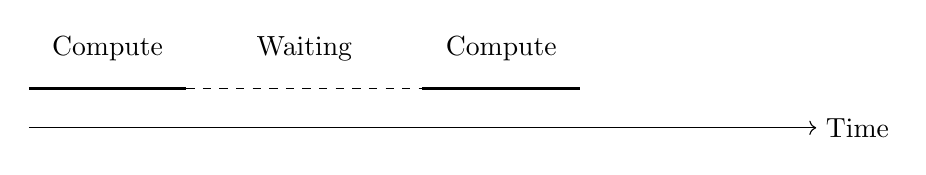
\begin{tikzpicture}
		\draw[->] (0,0) -- (10,0) node[right]{Time};
		
		\draw[thick] (0,0.5) -- (2,0.5);
		\draw[dashed] (2,0.5) -- (5,0.5);
		\draw[thick] (5,0.5) -- (7,0.5);
		
		\node at (1,1) {Compute};
		\node at (3.5,1) {Waiting};
		\node at (6,1) {Compute};
	\end{tikzpicture}
\end{center}


% ------------------------------------------------------------
\subparagraph{1) Pain Demo Part 1: The Queue Forms (20 min)}

\textbf{Demo setup (transparent to students)}\\
\textbf{Show the code first (2 minutes):}
\begin{lstlisting}[language=Java]
	// Single-threaded server (simplified)
	while (true) {
		Request req = acceptConnection();
		processRequest(req);  // includes Thread.sleep(100) to simulate DB call
		sendResponse(req);
	}
\end{lstlisting}

\textbf{Important clarification:}
The 100ms sleep simulates a blocking database or external API call.
The CPU is idle during this time.

\textbf{Ask students immediately:}
\begin{quote}
	Is the server slow because the CPU is weak?
\end{quote}

% ------------------------------------------------------------
\textbf{Live Demo Sequence}

\begin{itemize}[leftmargin=*]
	
	\item \textbf{Step 1: Baseline (1 client)}
	
	\begin{itemize}[leftmargin=*]
		\item Send 1 request $\rightarrow$ response time $\approx 100$ms
		\item CPU usage: $\approx 0\%$
		\item Compute time: $\approx 1$--$2$ms
		\item Waiting time: $\approx 98$ms
	\end{itemize}
	
	\textbf{Board calculation:}
	
	\[
	\text{CPU Utilization} = \frac{\text{Compute Time}}{\text{Total Time}}
	= \frac{2}{100} = 2\%
	\]
	
	\textbf{Punchline:}
	Server is idle 98\% of the time.
	
	\item \textbf{Step 2: Light load (5 concurrent clients)}
	
	\begin{itemize}[leftmargin=*]
		\item All arrive at $t=0$
		\item Sequential handling
		\item Latency $\approx 5 \times 100$ms = 500ms
		\item CPU still $\approx 2\%$
	\end{itemize}
	
	\textbf{Ask:}
	Why does latency multiply if CPU is not busy?
	
	\item \textbf{Step 3: Breaking point (50 concurrent clients)}
	
	\begin{itemize}[leftmargin=*]
		\item Latency $\approx 50 \times 100$ms = 5000ms
		\item CPU still mostly idle
	\end{itemize}
	
	\textbf{Punchline:}
	This is \textbf{I/O-bound starvation}.
	The CPU is free. The architecture is wrong.
	
\end{itemize}

% ------------------------------------------------------------
\textbf{Instructor-Led Mathematical Analysis}

We model the system formally.

Each request requires:
\[
T_{compute} = 2ms
\]
\[
T_{wait} = 98ms
\]

Total:
\[
T_{service} = 100ms
\]

Arrival burst:
\[
\lambda = 50 \text{ requests at } t=0
\]

Sequential server → behaves like M/M/1 with blocking.

Little's Law intuition:

\[
L = \lambda W
\]

If service time $W = 5s$ under burst load:

\[
L = 50
\]

All 50 requests are stuck inside the system.

% ------------------------------------------------------------
\textbf{Timeline Visualization}

(draw TikZ as you already prepared)

% ------------------------------------------------------------
\textbf{Critical Thinking Question}

What percentage of total time is productive computation?

\[
\frac{2}{100} = 2\%
\]

\textbf{Follow-up question:}
If CPU is idle 98\% of the time,
what is the real bottleneck?

Expected answer:
Blocking I/O.

% ------------------------------------------------------------
\textbf{Mini In-Class Exercise (3 min)}

If sleep becomes 200ms instead of 100ms:

\begin{enumerate}
	\item What happens to latency for 50 clients?
	\item What happens to CPU utilization?
\end{enumerate}

\textbf{Expected reasoning:}

Latency:
\[
50 \times 200ms = 10s
\]

CPU utilization:
\[
\frac{2}{200} = 1\%
\]

Doubling wait time halves CPU utilization.

\textbf{Conclusion:}
The system is not CPU-bound.
It is waiting-bound.

% ------------------------------------------------------------
\textbf{Transition Statement}

\begin{quote}
	If the CPU is idle 98\% of the time,
	why do we allow it to serve only one request?
\end{quote}

This is the birth of concurrency.


% ------------------------------------------------------------
\subparagraph{2) Conceptual Foundation (30 min)}
\textbf{Goal:} Give students the vocabulary + mental models to explain what they just observed.

% ============================================================
\subsubsection*{Concept 1: Latency vs Throughput (10 min)}
% ============================================================

\textbf{Warm-up prompt (1 min):}
\begin{quote}
	A system can be ``fast'' in two different ways. What are they?
\end{quote}

\textbf{Interactive exercise (5 min):}
\begin{itemize}[leftmargin=*]
	\item \textbf{Server A:} completes each request in 50ms, but can only handle 10 requests/second.
	\item \textbf{Server B:} completes each request in 5000ms, but can also handle 10 requests/second.
	\item \textbf{Question:} Which server would you rather use as a human? Why?
\end{itemize}

\textbf{Expected student insight:}
Humans care first about \textbf{latency}. Businesses often care about \textbf{throughput}.

\textbf{Definitions (emerge from answers):}
\begin{itemize}[leftmargin=*]
	\item \textbf{Latency:} time to finish \textit{one} request (user-facing).
	\item \textbf{Throughput:} requests completed per second (system/business metric).
\end{itemize}

\textbf{One-line reality check:}
\begin{quote}
	A system can have high throughput while still feeling slow (high latency).
\end{quote}

\textbf{Micro-example (board, 1 min):}
If a single-threaded server takes $100$ms per request, then:
\[
\text{Throughput}_{max} \approx \frac{1}{0.1} = 10 \text{ req/s}
\]
But under burst load, latency grows linearly.

\textbf{Visual aid: Restaurant analogy (2 min):}
\begin{itemize}[leftmargin=*]
	\item \textbf{Fast food:} low latency, high throughput
	\item \textbf{Fine dining:} high latency, low throughput
	\item \textbf{Festival food truck:} throughput stays high, but lines create high latency (what we just saw)
\end{itemize}

\textbf{Checkpoint question (30 sec):}
\begin{quote}
	Which metric does a user feel immediately: latency or throughput?
\end{quote}

% ============================================================
\subsubsection*{Concept 2: Concurrency vs Parallelism (10 min)}
% ============================================================

\textbf{Definitions:}
\begin{itemize}[leftmargin=*]
	\item \textbf{Concurrency:} managing many tasks at once (interleaving, scheduling, structure).
	\item \textbf{Parallelism:} executing tasks at the same time (requires multiple cores).
\end{itemize}

\textbf{Critical insight (say it slowly):}
\begin{quote}
	Concurrency is about \textbf{structure}. Parallelism is about \textbf{execution}.
\end{quote}

\textbf{Mini-demo (2 min):}
Show Task Manager / \texttt{htop}:
\begin{itemize}[leftmargin=*]
	\item Many threads exist
	\item Only a few run at any instant
	\item Scheduler switches among them (illusion of simultaneity)
\end{itemize}

\textbf{Pair exercise (2 min):}
\begin{quote}
	A single-core CPU running 10 threads: concurrent, parallel, both, or neither?
\end{quote}

\textbf{Expected answer:} \textbf{Concurrent only} (interleaving, not simultaneous execution).

\textbf{Instructor clarification (1 min):}
\begin{itemize}[leftmargin=*]
	\item One core $\Rightarrow$ at most one thread runs at a time $\Rightarrow$ no true parallelism.
	\item But concurrency can still improve responsiveness when tasks spend time waiting.
\end{itemize}

% ============================================================
\subsubsection*{Concept 3: I/O Wait vs CPU Work (10 min)}
% ============================================================

\textbf{The ratio that matters:}
\[
T_{service} = T_{cpu} + T_{io}
\]

\textbf{Typical profiles (context, not memorization):}
\begin{itemize}[leftmargin=*]
	\item \textbf{I/O-bound:} web servers, databases, file services (often 80--95\% waiting)
	\item \textbf{CPU-bound:} video encoding, ML training, large crypto operations
\end{itemize}

\textbf{Guiding question (2 min):}
\begin{quote}
	If 90\% of request time is I/O wait, what happens when you add 8 CPU cores?
\end{quote}

\textbf{Expected answer:}
Almost nothing for that request, because extra cores do not reduce waiting time.

\textbf{Light theoretical hook (Amdahl preview, 2 min):}
If only 10\% is CPU work (parallelizable part is limited), then speedup has a hard ceiling:
\[
S_{max} \approx \frac{1}{0.9} \approx 1.11
\]
Even ``infinite cores'' cannot make waiting disappear.

\textbf{Closing statement (tie back to demo):}
\begin{quote}
	Concurrency helps most when systems spend most of their time waiting.
\end{quote}

\textbf{Transition question (to next section):}
\begin{quote}
	So what is the simplest way to overlap waiting time for many clients?
\end{quote}
(Expected: threads / async I/O / event loop.)




% ============================================================
\subsubsection*{Theoretical Framing: Why Concurrency Works (and Fails)}
% ============================================================

Practical systems fail for mathematical reasons.

Before adding threads blindly, we must understand three foundational principles:

\begin{itemize}
	\item Amdahl's Law (Limits of Speedup)
	\item Little's Law (Queue Behavior)
	\item Context Switching Cost (Hidden Overhead)
\end{itemize}

% ------------------------------------------------------------
\paragraph{1) Amdahl's Law --- The Limit of Parallel Speedup}

Amdahl's Law states that the maximum theoretical speedup of a program is limited by the fraction that must run sequentially.

\[
S(N) = \frac{1}{(1 - P) + \frac{P}{N}}
\]

Where:
\begin{itemize}
	\item $P$ = parallelizable fraction
	\item $N$ = number of threads/processors
	\item $S(N)$ = maximum speedup
\end{itemize}

\textbf{Example:}

Suppose:
\begin{itemize}
	\item 80\% of the server work is waiting or parallelizable ($P=0.8$)
	\item 20\% must remain sequential
\end{itemize}

With 10 threads:

\[
S(10) = \frac{1}{0.2 + \frac{0.8}{10}}
= \frac{1}{0.2 + 0.08}
= \frac{1}{0.28}
\approx 3.57
\]

Even with 10 threads, the maximum speedup is only 3.57×.

\textbf{Important:}
Even infinite threads cannot exceed:

\[
\frac{1}{1-P}
\]

In this case:

\[
\frac{1}{0.2} = 5
\]

Theoretical upper bound = 5× speedup.

Concurrency improves performance,
but mathematics imposes a ceiling.

% ------------------------------------------------------------
\paragraph{2) Little's Law --- Why Queues Form}

Little's Law relates:

\[
L = \lambda W
\]

Where:
\begin{itemize}
	\item $L$ = average number of requests in system
	\item $\lambda$ = arrival rate (requests per second)
	\item $W$ = average time in system
\end{itemize}

\textbf{Example:}

If:
\begin{itemize}
	\item 50 requests per second arrive ($\lambda=50$)
	\item Each request takes 200ms = 0.2s
\end{itemize}

Then:

\[
L = 50 \times 0.2 = 10
\]

There will be 10 concurrent requests inside the system on average.

If you only allow 1 thread:

Queue grows immediately.

Little's Law explains:
\begin{quote}
	High latency automatically increases queue size.
\end{quote}

Concurrency reduces waiting time by overlapping execution.

% ------------------------------------------------------------
\paragraph{3) Context Switching Cost --- Why Threads Hurt}

Threads are not free.

Each context switch involves:

\begin{itemize}
	\item Saving registers
	\item Flushing CPU pipelines
	\item Possible cache invalidation
\end{itemize}

Assume:
\begin{itemize}
	\item Context switch cost = 5 microseconds
	\item 100,000 switches per second
\end{itemize}

Overhead:

\[
100{,}000 \times 5 \mu s = 500{,}000 \mu s = 0.5s
\]

Half the CPU time is wasted switching!

Too many threads reduce throughput.

Concurrency helps until scheduling overhead dominates.

% ------------------------------------------------------------
\paragraph{Synthesis}

\begin{itemize}
	\item Amdahl: Parallelism has a limit.
	\item Little: Waiting increases queue size.
	\item Context switching: Too many threads reduce performance.
\end{itemize}

Concurrency is a balance between:
\begin{center}
	Idle time exploitation \quad vs \quad Scheduling overhead.
\end{center}

Engineers must measure before optimizing.


\textbf{Concrete example:}
\begin{itemize}[leftmargin=*]
	\item 90\% parallelizable, infinite cores $\Rightarrow$ max speedup $= 1/0.1 = 10\times$
\end{itemize}

\textbf{Student calculation:}\\
\textit{``If 50\% is parallelizable, what's the max speedup with 100 cores?''}\\
\textbf{Expected answer:} $\approx 2\times$

\textbf{Key takeaway (write on board):}\\
\textit{``You cannot parallelize waiting away. You must hide it.''}

% ------------------------------------------------------------
\subparagraph{3) Transition Activity: Predict--Then--Test (15 min)}

\textbf{Scenario:} ``We're about to add threads. Predict what will happen to:''

\begin{enumerate}[leftmargin=*]
\item Latency (p50)
\item Throughput
\item CPU usage
\end{enumerate}

Students write predictions (1 min).\\
Reveal answer in Session 2.

% ------------------------------------------------------------
\subparagraph{4) Common Misconceptions Quiz (10 min)}

\textbf{True/False (with defense in pairs):}
\begin{enumerate}[leftmargin=*]
\item ``High throughput always means low latency.'' (False)
\item ``Adding more threads always improves performance.'' (False)
\item ``Parallelism requires multiple cores; concurrency does not.'' (True)
\item ``If CPU is at 10\%, the system is underutilized.'' (Depends)
\item ``Concurrency is only useful for I/O-bound tasks.'' (Mostly true; nuanced)
\end{enumerate}

% ------------------------------------------------------------
\subparagraph{5) Session 1 Wrap + Homework Bridge (10 min)}

\textbf{Summary (students repeat back):}
\begin{itemize}[leftmargin=*]
\item Concurrency $\neq$ speed; concurrency = hide waiting
\item Latency $\neq$ throughput (both matter)
\item Most servers are I/O-bound
\end{itemize}

\textbf{Before next session:}
\begin{itemize}[leftmargin=*]
\item Review the demo code (posted)
\item Think: ``How would you fix the waiting problem?''
\end{itemize}

\textbf{Exit ticket (2 min):}
\begin{enumerate}[leftmargin=*]
\item Define latency in one sentence.
\item Why is CPU low when latency is high?
\item True/False: More threads always help.
\end{enumerate}

% ============================================================
\paragraph{Session 2 (2h) --- ``The Fix \& The New Problem''}

\subparagraph{0) Recap + Answer Reveal (5 min)}
Revisit predictions from Session 1 and compare with measured outcomes.

% ------------------------------------------------------------
\subparagraph{1) Pain Demo Part 2: Multi-Threaded Server (25 min)}

\textbf{Demo setup (show new code):}
\begin{lstlisting}[language=Java]
ExecutorService pool = Executors.newFixedThreadPool(10);

while (true) {
	Request req = acceptConnection();
	pool.submit(() -> {
		processRequest(req);  // still 100ms sleep
		sendResponse(req);
	});
}
\end{lstlisting}

\textbf{Key change:} ``Now 10 requests can wait simultaneously.''

\textbf{Live demo sequence}
\begin{itemize}[leftmargin=*]
\item \textbf{Test 1: Same 50 clients}
\begin{itemize}[leftmargin=*]
	\item Latency drops from $\sim$5000ms $\rightarrow$ $\sim$500ms
	\item Throughput: $\sim$10$\times$ improvement
	\item CPU still low (still I/O-bound)
	\item \textbf{Punchline:} ``Hiding waiting works.''
\end{itemize}
\item \textbf{Demo twist: Push to failure}
\begin{itemize}[leftmargin=*]
	\item Test 2: 200 clients, pool size 10 $\rightarrow$ latency spikes again (queue forms)
	\item Test 3: increase pool to 200 $\rightarrow$ initial improvement, then degradation
\end{itemize}
\end{itemize}

\textbf{Example table to show:}
\begin{verbatim}
Pool size | Latency p95 | Throughput | CPU
10        | 500ms       | 100/sec    | 5%
50        | 200ms       | 250/sec    | 15%
200       | 300ms       | 200/sec    | 40%  <- worse!
500       | 1000ms      | 150/sec    | 60%  <- much worse!
\end{verbatim}

\textbf{Key realization:}\\
\textit{``Threads are not free. There is a sweet spot.''}

% ------------------------------------------------------------
\subparagraph{2) Analysis: Why Threads Helped (15 min)}

\textbf{Timeline comparison (board)}

\textbf{Single-threaded:}
\begin{verbatim}
t=0    t=100  t=200  t=300  ...  t=4900
|req1| |req2| |req3|           |req50|
\end{verbatim}

\textbf{Multi-threaded (pool=10):}
\begin{verbatim}
t=0    t=100  t=200  t=300  t=400  t=500
|req1|
|req2|
...
|req10|
|req11|
|req12|
...
\end{verbatim}

\textbf{Calculation:}
\begin{itemize}[leftmargin=*]
\item Single: $50 \times 100$ms = 5000ms for last client
\item Pooled (10): 5 batches $\times 100$ms = 500ms for last client
\end{itemize}

\textbf{Why it worked:} overlapped waiting periods; used time previously idle.

% ------------------------------------------------------------
\subparagraph{3) Analysis: Why Too Many Threads Hurt (15 min)}

\textbf{Sources of overhead}
\begin{itemize}[leftmargin=*]
\item \textbf{Context switching cost:} with hundreds of threads on few cores, scheduler thrashes
\item \textbf{Memory overhead:} each thread has a stack; large thread counts waste memory
\item \textbf{Contention:} threads compete for shared resources (locks, scheduler, queues)
\end{itemize}

\textbf{Rule of thumb (write large):}
\begin{quote}
	\[
	\textbf{Optimal thread count} \approx
	\textbf{cores}\times\left(1+\frac{\text{wait time}}{\text{compute time}}\right)
	\]
\end{quote}


Example:
\begin{itemize}[leftmargin=*]
\item wait/compute = 90/10 = 9
\item 8 cores $\times (1 + 9)$ = 80 threads (not 500)
\end{itemize}

% ------------------------------------------------------------
\subparagraph{4) Case Study: Redis \& SQLite (15 min)}

\textbf{Prompt:} ``Given what we learned, why choose single-threaded designs?''

\textbf{Expected points:}
\begin{itemize}[leftmargin=*]
\item simpler (no races, fewer locks)
\item predictable latency
\item cache locality
\item single-threaded can still be extremely fast for in-memory workloads
\end{itemize}

\textbf{Key insight:}\\
\textit{``Engineering is tradeoffs. Single-threaded is a choice, not a limitation.''}

% ------------------------------------------------------------
\subparagraph{5) Lab 1.1 Briefing (30 min)}

\textbf{What students must submit:}

\textbf{(1) Measurements table:}

% ------------------------------------------------------------
% Measurements Table (TikZ) — Throughput columns wider
% ------------------------------------------------------------
\begin{center}
	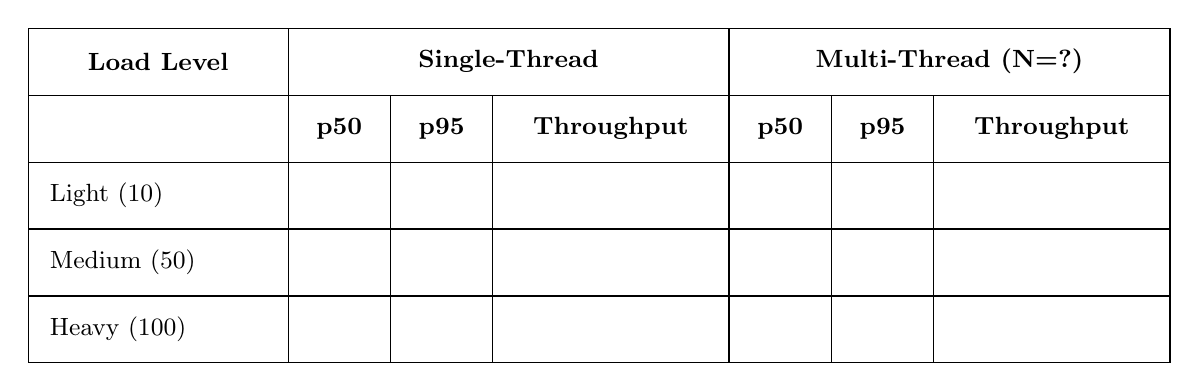
\begin{tikzpicture}[font=\small]
		% ---- Table geometry ----
		\def\wA{3.3}   % Load Level column width
		\def\wB{5.6}   % Single-Thread group width (3 subcolumns, throughput wider)
		\def\wC{5.6}   % Multi-Thread group width (3 subcolumns, throughput wider)
		\def\h{0.85}   % row height
		
		% Total width
		\pgfmathsetmacro{\W}{\wA+\wB+\wC}
		
		% X positions (group boundaries)
		\pgfmathsetmacro{\xA}{\wA}
		\pgfmathsetmacro{\xB}{\wA+\wB}
		
		% ---- Unequal subcolumn widths: p50, p95, Throughput (wider) ----
		\def\sBp{1.3}                 % p50 (Single-Thread)
		\def\sBq{1.3}                 % p95 (Single-Thread)
		\pgfmathsetmacro{\sBr}{\wB-\sBp-\sBq}  % Throughput = remaining (Single-Thread)
		
		\def\sCp{1.3}                 % p50 (Multi-Thread)
		\def\sCq{1.3}                 % p95 (Multi-Thread)
		\pgfmathsetmacro{\sCr}{\wC-\sCp-\sCq}  % Throughput = remaining (Multi-Thread)
		
		% ---- Outer border (5 rows: header + subheader + 3 data rows) ----
		\draw (0,0) rectangle (\W, -5*\h);
		
		% ---- Horizontal lines ----
		\foreach \r in {1,2,3,4} {
			\draw (0,-\r*\h) -- (\W,-\r*\h);
		}
		
		% ---- Vertical lines (main group splits) ----
		\draw (\xA,0) -- (\xA,-5*\h);
		\draw (\xB,0) -- (\xB,-5*\h);
		
		% ---- Subcolumn vertical lines (start below first header row) ----
		% Single-Thread: after p50, after p95
		\draw (\xA+\sBp, -\h) -- (\xA+\sBp, -5*\h);
		\draw (\xA+\sBp+\sBq, -\h) -- (\xA+\sBp+\sBq, -5*\h);
		
		% Multi-Thread: after p50, after p95
		hi
		\draw (\xB+\sCp, -\h) -- (\xB+\sCp, -5*\h);
		\draw (\xB+\sCp+\sCq, -\h) -- (\xB+\sCp+\sCq, -5*\h);
		
		% ---- Header row (row 1) ----
		\node[align=center] at (\wA/2, -0.5*\h) {\textbf{Load Level}};
		\node[align=center] at (\xA+\wB/2, -0.5*\h) {\textbf{Single-Thread}};
		\node[align=center] at (\xB+\wC/2, -0.5*\h) {\textbf{Multi-Thread (N=?)}}; % edit N later
		
		% ---- Subheader row (row 2) ----
		% Single-Thread labels
		\node[align=center] at (\xA+0.5*\sBp, -1.5*\h) {\textbf{p50}};
		\node[align=center] at (\xA+\sBp+0.5*\sBq, -1.5*\h) {\textbf{p95}};
		\node[align=center] at (\xA+\sBp+\sBq+0.5*\sBr, -1.5*\h) {\textbf{Throughput}};
		
		% Multi-Thread labels
		\node[align=center] at (\xB+0.5*\sCp, -1.5*\h) {\textbf{p50}};
		\node[align=center] at (\xB+\sCp+0.5*\sCq, -1.5*\h) {\textbf{p95}};
		\node[align=center] at (\xB+\sCp+\sCq+0.5*\sCr, -1.5*\h) {\textbf{Throughput}};
		
		% ---- Data rows (rows 3..5) ----
		\node[anchor=west] at (0.15, -2.5*\h) {Light (10)};
		\node[anchor=west] at (0.15, -3.5*\h) {Medium (50)};
		\node[anchor=west] at (0.15, -4.5*\h) {Heavy (100)};
		
	\end{tikzpicture}
\end{center}


\textbf{(2) Concurrency scorecard:}
\begin{verbatim}
[ ] Thread-safe? (if shared state exists, is it protected?)
[ ] Visibility guaranteed? (N/A for basic server)
[ ] Deadlock-free? (N/A for basic server)
[ ] Liveness guaranteed? (are requests eventually served?)
[ ] Bounded resources? (did you cap thread pool? queue?)
[ ] Failure recovery path? (timeouts? retries? or none?)
\end{verbatim}

\textbf{(3) Explanation paragraph (5--8 sentences)} using rubric language:
\begin{itemize}[leftmargin=*]
\item mechanism changed (threads)
\item why performance improved (hiding I/O wait)
\item tradeoff introduced (resource overhead, complexity)
\end{itemize}

\textbf{Starter structure (show):}
\begin{verbatim}
	lab1/
	|-- single_threaded_server.java
	|-- multi_threaded_server.java
	|-- client.java (load generator)
	|-- README.md (how to run)
	`-- measurements_template.md
\end{verbatim}


\textbf{How to run tests:}
\begin{lstlisting}[language=bash]
# Terminal 1: Start server
java SingleThreadedServer 8080

# Terminal 2: Run load test
java Client localhost 8080 --clients=50 --requests=10

# Output: CSV with latencies
\end{lstlisting}

\textbf{Common pitfalls:}
\begin{itemize}[leftmargin=*]
\item Not warming up (JVM warmup): discard first 10--20 measurements
\item Server and client on same machine: acceptable, but must be noted
\item Thread pool size = client count: defeats the purpose; test multiple sizes (5, 10, 20, 50)
\end{itemize}

% ------------------------------------------------------------
\subparagraph{6) Hands-On Exercise: Predict Optimal Pool Size (10 min)}

\textbf{Scenario:}
\begin{itemize}[leftmargin=*]
\item 8-core machine
\item request profile: 90\% I/O wait, 10\% CPU
\item target: 100 concurrent clients
\end{itemize}

\textbf{Question:} ``What pool size would you try first? Why?''

\textbf{Calculation together:}
\begin{verbatim}
wait/compute = 90/10 = 9
optimal $\approx$ 8 × (1 + 9) = 80 threads
Try pool sizes: 20, 40, 60, 80
Measure and find the knee of the curve
\end{verbatim}

% ------------------------------------------------------------
\subparagraph{7) Common Mistakes + Misconceptions (10 min)}

\begin{itemize}[leftmargin=*]
\item ``More threads = faster'' (false; demonstrated)
\item ``High throughput means good UX'' (false; latency matters)
\item ``Parallelism and concurrency are the same'' (false)
\item ``If CPU is low, the system is underutilized'' (depends; I/O-bound is expected)
\end{itemize}

% ------------------------------------------------------------
\subparagraph{8) Session 2 Wrap + Next Week Preview (10 min)}

\textbf{Summary (students state aloud):}
\begin{itemize}[leftmargin=*]
\item Threads hide waiting by overlapping I/O
\item Too many threads introduce overhead
\item Engineering is finding the sweet spot
\end{itemize}

\textbf{Next week teaser:}\\
\textit{``Thread pools work great... until they don't. Next week: what breaks when threads share data.''}

\textbf{Final thought (board):}
\begin{verbatim}
Concurrency is not speed.
Concurrency is hiding waiting.

But hiding waiting creates new problems.
\end{verbatim}

% ============================================================
\subsubsection*{Additional Materials Needed}

\textbf{1) Slide deck outline (12 slides max):}
\begin{enumerate}[leftmargin=*]
\item Title + Course context
\item Learning targets
\item Demo 1 setup (code snippet)
\item Demo 1 results (clients vs latency)
\item Latency vs throughput (definitions + example)
\item Concurrency vs parallelism (definitions + visual)
\item Amdahl's law (formula + example)
\item Demo 2 setup (code snippet)
\item Demo 2 results (comparison table)
\item Why threads hurt (overhead sources)
\item Lab 1.1 deliverables checklist
\item Week 1 summary + Week 2 preview
\end{enumerate}

\vspace{1mm}
\textbf{2) Grading rubric for Lab 1.1:}

\textbf{Measurements table (30\%):}
\begin{itemize}[leftmargin=*]
\item[$\square$] All cells filled (10\%)
\item[$\square$] Reasonable values (10\%)
\item[$\square$] Multiple load levels tested (10\%)
\end{itemize}

\textbf{Concurrency scorecard (20\%):}
\begin{itemize}[leftmargin=*]
\item[$\square$] All items addressed (10\%)
\item[$\square$] Honest assessment (not all ``yes'') (10\%)
\end{itemize}

\textbf{Explanation paragraph (40\%):}
\begin{itemize}[leftmargin=*]
\item[$\square$] Mechanism described (10\%)
\item[$\square$] Performance change explained (10\%)
\item[$\square$] Tradeoff identified (10\%)
\item[$\square$] Uses rubric language (10\%)
\end{itemize}

\textbf{Code quality (10\%):}
\begin{itemize}[leftmargin=*]
\item[$\square$] Runs without modification (5\%)
\item[$\square$] Reasonable structure (5\%)
\end{itemize}

\textbf{Total: /100}

\vspace{1mm}
\textbf{3) Pre-lab checklist (student-facing):}

\textbf{Before Lab 1.1:}
\begin{itemize}[leftmargin=*]
\item[$\square$] Reviewed demo code from lecture
\item[$\square$] Java development environment set up
\item[$\square$] Can run provided starter code
\item[$\square$] Understand how to measure latency (p50/p95)
\item[$\square$] Know how to monitor CPU usage
\end{itemize}

\textbf{During Lab 1.1:}
\begin{itemize}[leftmargin=*]
\item[$\square$] Warm up runtime before measurements
\item[$\square$] Test at least 3 different load levels
\item[$\square$] Try at least 3 different thread pool sizes
\item[$\square$] Record CPU observations for each test
\item[$\square$] Fill scorecard honestly (not all boxes checked)
\end{itemize}

\textbf{After Lab 1.1:}
\begin{itemize}[leftmargin=*]
\item[$\square$] Compare single vs multi-threaded results
\item[$\square$] Identify optimal thread pool size
\item[$\square$] Write explanation using rubric language
\item[$\square$] Proofread before submission
\end{itemize}

% ============================================================
\subsubsection*{Key Improvements Over Original Plan}

\begin{enumerate}[leftmargin=*]
\item Exit tickets + entrance tickets for formative assessment
\item Predict--then--test for active learning
\item Concrete calculations (Amdahl + pool sizing rule of thumb)
\item Failure demonstration (limits, not just success)
\item Rubric alignment from day 1 (quality language early)
\item Preparation checklist (reduces ``how do I start'' issues)
\item Memory aids (``Concurrency is hiding waiting'' repeated)
\item Two-session split with cliffhanger to maintain engagement
\item Real-world anchors (Redis, restaurant analogy)
\item Explicit misconception destruction
\end{enumerate}

% ============================================================
\subsubsection*{Instructor Self-Checklist}

\textbf{Before Week 1:}
\begin{itemize}[leftmargin=*]
\item[$\square$] Demo code tested on classroom machine
\item[$\square$] Backup demos recorded
\item[$\square$] Starter code repository accessible
\item[$\square$] Grading rubric posted
\item[$\square$] Exit ticket questions printed/digital
\end{itemize}

\textbf{During Session 1:}
\begin{itemize}[leftmargin=*]
\item[$\square$] Students can see terminal + system monitor simultaneously
\item[$\square$] Exit ticket collected
\item[$\square$] Demo code shared immediately after class
\end{itemize}

\textbf{During Session 2:}
\begin{itemize}[leftmargin=*]
\item[$\square$] Predictions revisited
\item[$\square$] Lab deliverables crystal clear
\item[$\square$] Students leave knowing how to start
\end{itemize}

\textbf{After Week 1:}
\begin{itemize}[leftmargin=*]
\item[$\square$] Lab submissions graded with rubric
\item[$\square$] Common mistakes noted for Week 2 opening
\item[$\square$] Optimal thread pool sizes from student data collected (reuse in Week 5)
\end{itemize}
	
	
\end{document}